\chapter{Background} \label{ch:background}



This chapter introduces the background needed for the methods developed in Chapters~\ref{ch:mcmc} and \ref{ch:simplex}.  We start by giving a brief introduction to Riemannian geometry, then introducing methods for approximate Bayesian inference and finally approaches for modeling discrete data. 

\section{Basic notions in Riemannian Geometry} \label{sec:riemannian_background}
For a formal and rigorous introduction to Riemannian geometry we refer the reader to \citet{do1992riemannian} and \citet{Lee2018}. Here we introduce only the concepts needed later in the thesis, under simplified settings that cover our examples. We consider manifolds that admit a global chart, a subset of which are  smooth embedded submanifolds of Euclidean space. This allows us to write the coordinates globally, and avoid dealing with local coordinates patches. When the space has a boundary (e.g. the simplex) we consider the differential geometric objects only on the interior of the space. 

\subsection{Riemannian manifolds}

\paragraph{Manifolds and tangent spaces}
A smooth $D$-dimensional manifold $\mathcal{M}$ is a topological space that is
locally diffeomorphic to $\mathbb{R}^D$. For the manifolds we consider, we assume that
$\mathcal{M}$ admits a global chart $\varphi:\mathcal{M}\to U\subseteq\mathbb{R}^D$
with inverse $\psi=\varphi^{-1}$. For $\boldsymbol{x} \in \mathcal{M}$, we denote its coordinates by
$\boldsymbol{z} =  \varphi(\boldsymbol{x}) \in U$, where $z^j:\mathcal{M}\to\mathbb{R}$
denotes the $j$-th coordinate function, i.e.\ $\varphi(\boldsymbol{x}) = (z^1(\boldsymbol{x}),\dots,z^D(\boldsymbol{x}))$.
The tangent space $T_{\boldsymbol{x}}\mathcal{M}$ is the vector space of velocities
of smooth curves that pass through $\boldsymbol{x}$. If
$\gamma:(-\varepsilon,\varepsilon)\to \mathcal{M}$, for some $\varepsilon>0$, is a smooth curve with
$\gamma(0)=\boldsymbol{x}$, define $\boldsymbol z(t):=\varphi(\gamma(t))$. Then
$\gamma(t)=\psi(\boldsymbol z(t))$, and by the chain rule
\[
\dot\gamma(0)
=
\sum_{i=1}^D \dot z^i(0)\,
\frac{\partial}{\partial z^i},
\]
where $\frac{\partial}{\partial z^i}
:=
\frac{\partial \psi}{\partial z^i}(\boldsymbol z)
\in T_{\boldsymbol x}\mathcal M$. The expression above shows that $\partial/\partial z^i$ span the tangent space. Moreover,
\[
\frac{\partial}{\partial z^i}(z^j)
=\frac{\partial (z^j\circ \psi)  }{\partial z^i} (\boldsymbol{z})
=\frac{\partial z^j  }{\partial z^i} 
=\delta_i^j,
\]
which implies linear independence, so $\left\{\frac{\partial}{\partial z^i}\right\}_{i=1}^D$ form a basis of $T_{\boldsymbol x}\mathcal M$.


\paragraph{Riemannian metric}
For two tangent vectors  $\boldsymbol{u},\boldsymbol{v}\in T_{\boldsymbol{x}}\mathcal{M}$, we write $\boldsymbol{u}=\sum_{i=1}^D u^i \frac{\partial}{\partial z^i},
\boldsymbol{v}=\sum_{i=1}^D v^i \frac{\partial}{\partial z^i}$.
The Riemannian metric defines for each $\boldsymbol{x}\in\mathcal{M}$ an inner product on the tangent space $g:T_{\boldsymbol{x}}\mathcal{M} \times T_{\boldsymbol{x}}\mathcal{M} \to \mathbb{R}$.
We represent it with a symmetric positive definite matrix $\mathbf{G}(\boldsymbol{x})$ 
with $G_{ij}(\boldsymbol{x}) = g_{\boldsymbol{x}}(\partial/\partial z^i,\partial/\partial z^j)$,
such that 
\begin{equation*}
g_{\boldsymbol{x}}(\boldsymbol{u}, \boldsymbol{v}) = 
\langle \boldsymbol{u},\boldsymbol{v}\rangle_{\mathbf{G}(\boldsymbol{x})}
=
\boldsymbol{u}^\top \mathbf{G}(\boldsymbol{x})\boldsymbol{v},
\end{equation*}
where on the right-hand side $\boldsymbol{u}=(u^1,\dots,u^D)^\top$ and
$\boldsymbol{v}=(v^1,\dots,v^D)^\top$ denote the vector components. 
This metric defines lengths of tangent vectors, lengths of curves, angles, and geodesic distance. A manifold endowed with a metric tensor is called a \emph{Riemannian manifold} and denoted by $(\mathcal{M}, g)$.

\paragraph{Embedded manifolds and the pullback metric}
Some of the mani-folds we consider are smooth embedded submanifolds of  $\mathbb{R}^K$, where $K\geq D$. Let $\psi:U\subseteq\mathbb{R}^D\to \mathbb{R}^K$ be a smooth embedding and let $\mathcal{M}=\psi(U)$.
Then, for $\boldsymbol{x} = \psi(\boldsymbol{z})\in \mathcal{M}$, the tangent space is
\begin{equation*}
T_{\boldsymbol{x}}\mathcal{M}
=
\left\{
\mathbf{J}_{\psi}(\boldsymbol{z})\boldsymbol{v}
\;:\;
\boldsymbol{v}\in\mathbb{R}^D
\right\},
\end{equation*}
where  $\mathbf{J}_{\psi}$ is the Jacobian matrix of  $\psi$. 
The ambient inner product induces a Riemannian metric on $\mathcal{M}$ by restriction to the tangent space.
If $\boldsymbol{u},\boldsymbol{v}\in T_{\boldsymbol{x}}\mathcal{M}$, 
such that $\boldsymbol{u} = \mathbf{J}_{\psi}(\boldsymbol{z}) \boldsymbol{a}$ and $\boldsymbol{v} = \mathbf{J}_{\psi}(\boldsymbol{z}) \boldsymbol{b}$ for $\boldsymbol{a}, \boldsymbol{b}\in \mathbb{R}^D$,
then
$g_{\boldsymbol{z}}(\boldsymbol{u},\boldsymbol{v})=\langle \boldsymbol{u},\boldsymbol{v}\rangle_2 = 
 \boldsymbol{a}^\top \mathbf{J}_{\psi}(\boldsymbol{z})^\top \mathbf{J}_{\psi}(\boldsymbol{z}) \boldsymbol{b}
$.
In coordinates $\boldsymbol{z}\in U$, this induced metric is represented by the matrix
\begin{equation*}
\mathbf{G}(\boldsymbol{z})
=
\mathbf{J}_{\psi}(\boldsymbol{z})^\top \mathbf{J}_{\psi}(\boldsymbol{z}).
\end{equation*}
Let us consider a classic example. The graph of a smooth function $f:\mathbb{R}^D\to\mathbb{R}$ is
\begin{equation*}
\mathcal{G}_f
:=
\left\{
(\boldsymbol{z},f(\boldsymbol{z})):\;
\boldsymbol{z}\in\mathbb{R}^D
\right\}
\subset \mathbb{R}^{D+1},
\end{equation*}
the embedding is $\psi(\boldsymbol{z})=(\boldsymbol{z},f(\boldsymbol{z}))$, so the induced metric is
\begin{equation*}
\mathbf{G}(\boldsymbol{z})
=
\mathbf{I}_D+\nabla f(\boldsymbol{z})\nabla f(\boldsymbol{z})^\top.
\end{equation*}
If $f(\boldsymbol{z})=\alpha \ell(\boldsymbol{z})$ for a log density $\ell$ and
tempering parameter $\alpha\geq 0$, this is the Monge metric (see Chapter~\ref{ch:mcmc}).
The different manifolds considered in this thesis are summarized in Table~\ref{tab:manifolds}.
\begin{table}[t]
\centering
\footnotesize
\renewcommand{\arraystretch}{1.2}
\begin{tabular}{@{}p{0.14\linewidth}p{0.52\linewidth}cc@{}}
\toprule
\textbf{Name} & \textbf{Definition} & \textbf{Embedded} & \textbf{Metric} \\
\midrule
Sphere &
$\mathbb{S}_{+}^{D}:=\{\boldsymbol{x}\in\mathbb{R}_{\ge 0}^{K}:\sum_{k=1}^{K} x_k^2 = 1\}$ &
$\checkmark$ &
Pullback \\
Simplex &
$\Delta^{D}:=\{\boldsymbol{x}\in\mathbb{R}_{\ge 0}^{K}:\sum_{k=1}^{K}x_k=1\}$ &
$\checkmark$ &
Custom \\
Graph &
$\mathcal{G}_{\alpha}:=\{(\boldsymbol{x},\alpha \ell(\boldsymbol{x})):\boldsymbol{x}\in\mathbb{R}^{D}\}$ &
$\checkmark$ &
Pullback \\
Statistical &
$\Theta:=\{\boldsymbol{x}\in\mathbb{R}^{D}:p_{\mathcal{Y}\mid\mathcal{X}}(\boldsymbol{y}\mid\boldsymbol{x})\,p_{\mathcal{X}}(\boldsymbol{x})>0\}$ &
-- &
Custom \\
\bottomrule
\end{tabular}
\caption{Summary of the manifolds considered in the thesis. In the case of the simplex and statistical manifolds we equip the space with custom choices of metric tensors presented in Chapters~\ref{ch:mcmc} and~\ref{ch:simplex}. }
\label{tab:manifolds}
\end{table}

\subsection{Geodesics}
The metric tensor defines the length of a smooth curve $\gamma:[0,1]\to\mathcal{M}$ by 
\begin{equation}
L(\gamma)
=
\int_0^1 \|\dot\gamma(t)\|_{\mathbf{G}(\gamma(t))}\,dt.
\end{equation}
A geodesic between two points $\boldsymbol{x}_0,\boldsymbol{x}_1\in\mathcal{M}$ is the curve that has the shortest length, namely
\begin{equation}
    d_g(\boldsymbol{x}_0,\boldsymbol{x}_1)
    =
    \inf_{\gamma}
    \int_0^1 \|\dot\gamma(t)\|_{\mathbf{G}(\gamma(t))}\,dt,
    \qquad
    \gamma(0)=\boldsymbol{x}_0,\ \gamma(1)=\boldsymbol{x}_1.
    \label{eq:geodesic_distance}
\end{equation}
A geodesic can equivalently be characterized as the curve with zero covariant acceleration, for this we need to define the notion of covariant derivative. 


\paragraph{Levi-Civita connection}
The Levi-Civita connection provides an intrinsic derivative of vector fields along tangent directions. It is the unique affine connection that is torsion free and compatible with the metric \citep{Lee2018}.
We use the notation $\partial_i := \partial/\partial z^i$. If $\boldsymbol{V}=\sum_{j=1}^D V^j\partial_j$ is a vector field and $\boldsymbol{u}=\sum_{i=1}^D u^i\partial_i\in T_{\boldsymbol{x}}\mathcal{M}$, then
\begin{equation*}
\nabla^{\mathbf{G}}_{\boldsymbol{u}}\boldsymbol{V}
=
\sum_{k=1}^D
\left(
\sum_{i=1}^D u^i \partial_i V^k
\;+\;
\sum_{i,j=1}^D \Gamma_{ij}^{k} u^i V^j
\right)\partial_k,
\end{equation*}
where $\Gamma^k_{ij}$ are the Christoffel symbols of the second kind 
\begin{equation} \label{eq:christoffel_symbols}
\Gamma^k_{ij}(\boldsymbol{x})
=
\frac{1}{2}\sum_{m=1}^D \mathbf{G}^{-1}_{km}(\boldsymbol{x})
\bigl(
\partial_i \mathbf{G}_{mj}(\boldsymbol{x})
+
\partial_j \mathbf{G}_{im}(\boldsymbol{x})
- \partial_m \mathbf{G}_{ij}(\boldsymbol{x})
\bigr). 
\end{equation}


\paragraph{Exponential map} 
A geodesic $\gamma$ has vanishing covariant acceleration, $\nabla^{\mathbf{G}}_{\dot{\gamma}(t)}\dot{\gamma}(t)=0$, this condition gives the following differential equation
\begin{equation}
\ddot{\gamma}^{k}(t)
+
\sum_{i,j=1}^{D}\Gamma_{ij}^{k}(\gamma(t))\dot{\gamma}^{i}(t)\dot{\gamma}^{j}(t)
=0,
\qquad k=1,\dots,D,
\label{eq:geodesic_equations}
\end{equation}
where we used 
$ \left( \sum_{i=1}^D \dot{\gamma}^{i}(t) \partial_i \right) \dot\gamma^k(t) = \dv[]{}{t} \dot\gamma^k(t) = \ddot{\gamma}^{k}(t)$.

For $\boldsymbol{x}\in\mathcal{M}$ and $\boldsymbol{v}\in T_{\boldsymbol{x}}\mathcal{M}$, let $\gamma_{\boldsymbol{x}, \boldsymbol{v}}$ be a geodesic with initial conditions $\gamma_{\boldsymbol{x}, \boldsymbol{v}}(0) = \boldsymbol{x}\in \mathcal{M}$ and $\dot \gamma_{\boldsymbol{x}, \boldsymbol{v}} =\boldsymbol{v}\in T_{\boldsymbol{x}}\mathcal{M}$. The exponential map is defined as 
\begin{equation*}
 \operatorname{Exp}_{\boldsymbol{x}}(t\boldsymbol{v}) = \gamma_{\boldsymbol{x}, \boldsymbol{v}}(t).
\end{equation*}
If the system does not have an analytical solution, the  exponential map is computed with numerical integration using standard ordinary differential equation solvers, such as Euler, or Dormand-Prince's method \citep{kidger2022neural}.

\paragraph{Logarithm map}
The logarithm map is the inverse of the exponential map. Given two sufficiently close positions $\boldsymbol{x}_0, \boldsymbol{x}_1 \in \mathcal{M}$ for which the inverse is well defined, it returns the velocity that generates the geodesic connecting them. This is a boundary value problem whose solution gives 
\begin{equation*}
    \boldsymbol{v} =\operatorname{Log}_{\boldsymbol{x}_0}(\boldsymbol{x}_1)\in T_{\boldsymbol{x}_0}\mathcal{M},
\end{equation*}
such that $\operatorname{Exp}_{\boldsymbol{x}_0}(\boldsymbol{v})=\boldsymbol{x}_1$.
If the solution is not computable analytically, the problem can be solved numerically by standard boundary value solvers, such as the solvers of \citet{2020SciPy-NMeth}. 

The main computational bottleneck comes from the computation of the Christoffel symbols since they involve the inverse metric and derivatives of the metric. The choice of numerical solver affects accuracy and runtime: fixed or adaptive step-size, and low to higher order solvers introduce tradeoff between stability, numerical error and computational cost. 


\subsection{Riemannian gradient and Hessian}
The notion of gradient and Hessian are modified such that they are consistent with the geometry introduced by  $\mathbf{G}(\boldsymbol{x})$. These quantities are introduced here and useful in Chapter~\ref{ch:mcmc}. 

\paragraph{Riemannian gradient}
Let $f:\mathcal{M}\to\mathbb{R}$ be a smooth function. The Riemannian gradient $\nabla_{\mathbf{G}}f(\boldsymbol{x})\in T_{\boldsymbol{x}}\mathcal{M}$ is a tangent vector which satisfies the identity
\begin{equation*}
    \langle \nabla_{\mathbf{G}} f(\boldsymbol{x}), \boldsymbol{v}\rangle_{\mathbf{G}(\boldsymbol{x})}
=
\mathrm{d}f_{\boldsymbol{x}}(\boldsymbol{v}),
\qquad \forall\, \boldsymbol{v}\in T_{\boldsymbol{x}}\mathbb{R}^D,
\end{equation*}
where the differential $\mathrm{d}f_{\boldsymbol{x}}:T_{\boldsymbol{x}}\mathbb{R}^D\to\mathbb{R}$ is such that $\mathrm{d}f_{\boldsymbol{x}}(\boldsymbol v)
=
\sum_{i=1}^D \frac{\partial f}{\partial z^i}(\boldsymbol{x})\, v^i$.
Solving for $\nabla_{\mathbf{G}}$, the Riemannian gradient has the components
\begin{equation}
(\nabla_{\mathbf{G}} f)^i
=
\sum_{j=1}^D \mathrm{G}^{ij}\,\partial_j f,
\label{eq:riemannian_gradient}
\end{equation}
where $\mathrm{G}^{ij}$ are the components of $\mathbf{G}^{-1}(\boldsymbol{x})$. 
If $f$ has support on $\mathcal{M}\subset\mathbb{R}^D$, the components are the Euclidean gradient scaled by the inverse metric. This quantity is sometimes referred to as the natural gradient \citep{amari1998natural}, in this case we can collect the components into the vector
\begin{equation*}
    \mathbf{G}(\boldsymbol{x})^{-1}\nabla_{\boldsymbol{x}}f, 
\end{equation*}
where $\nabla_{\boldsymbol{x}}f$ is the Euclidean gradient. 


\paragraph{Riemannian Hessian} 
The Riemannian Hessian is defined as the covariant derivative of the Riemannian gradient, for $\boldsymbol{x}\in\mathcal{M}$ and $\boldsymbol{v}\in T_{\boldsymbol{x}}\mathcal{M}$
\begin{equation*}
\mathrm{Hess}_{\mathbf{G}} f(\boldsymbol{x})[\boldsymbol{v}]
:=
\nabla^{\mathbf{G}}_{\boldsymbol{v}} \nabla_{\mathbf{G}} f.
\end{equation*}
This expression can be viewed as the vector with components
\begin{equation*}
\bigl(\mathrm{Hess}_{\mathbf{G}} f(\boldsymbol{x})[\boldsymbol{v}]\bigr)^i
=
\sum_{j=1}^D 
\sum_{m=1}^D \mathrm{G}^{im}\left(\partial_m\partial_j f
-
\sum_{k=1}^D \Gamma^k_{mj}\,\partial_k f\right)
\, v^j.
\end{equation*}
If $f$ has support on $\mathcal{M}\subset\mathbb{R}^D$, we can collect these components in the matrix
\begin{equation}
\mathbf{G}^{-1}(\boldsymbol{x})\left(\nabla^2 f(\boldsymbol{x})
- \sum_{k=1}^D \mathbf{\Gamma}^k(\boldsymbol{x})\,\partial_k f(\boldsymbol{x})\right)\boldsymbol{v},
\label{eq:riem_hessian}
\end{equation}
where $\nabla^2 f(\boldsymbol{x})$ is the Euclidean Hessian and $[\mathbf{\Gamma}^k(\boldsymbol{x})]_{ij} = {\Gamma}_{ij}^k(\boldsymbol{x})$. For Euclidean metric the Riemannian Hessian is a Hessian vector product. 


\section{Approximate Bayesian inference techniques}
Let $\mathcal{X}$ be a continuous random variable on $\mathbb{R}^D$ with smooth density $p_{\mathcal{X}}(\boldsymbol{x})$ with respect to the Lebesgue measure. Let $\boldsymbol{y}$ denote observed data, with likelihood $p_{\mathcal{Y}|\mathcal{X}}(\boldsymbol{y}\mid\boldsymbol{x})$. In Bayesian inference, the posterior density is
\begin{equation}
\underbrace{p_{\mathcal{X}|\mathcal{Y}}(\boldsymbol{x}\mid \boldsymbol{y})}_{\text{posterior}}
=
\frac{
\overbrace{ p_{\mathcal{Y}|\mathcal{X}}(\boldsymbol{y}\mid\boldsymbol{x})  }^{\text{likelihood}}
\;
\overbrace{ p_{\mathcal{X}}(\boldsymbol{x}) }^{\text{prior}}
}{
\underbrace{ p_{\mathcal{Y}}(\boldsymbol{y}) }_{\text{evidence}}
},
\label{eq:posterior}
\end{equation}
and the marginal likelihood or model evidence is
\begin{equation*}
    p_{\mathcal{Y}}(\boldsymbol{y})=\int_{\mathbb{R}^D} p_{\mathcal{Y}|\mathcal{X}}(\boldsymbol{y}\mid\boldsymbol{x})p_{\mathcal{X}}(\boldsymbol{x})\,d\boldsymbol{x}.
\end{equation*}
When the posterior falls on the same parametric family as the prior, the model is called conjugate and we do not need to rely on approximations. For example, we can compute expectations and credible intervals directly from this distribution. In most cases, however, $p_{\mathcal{Y}}(\boldsymbol{y})$ is intractable and we therefore work with the joint distribution $p_{\mathcal{X},\mathcal{Y}}(\boldsymbol{x},\boldsymbol{y})$. During posterior inference, $\boldsymbol{y}$ denotes observed data and is fixed. We work with the unnormalized target density
\begin{equation}
    p(\boldsymbol{x}) := p_{\mathcal{Y}|\mathcal{X}}(\boldsymbol{y}\mid\boldsymbol{x})\,p_{\mathcal{X}}(\boldsymbol{x}).
\end{equation}
Approximate Bayesian inference then relies on $p(\boldsymbol{x})$ or on its log-density $\ell(\boldsymbol{x}) := \log p(\boldsymbol{x})$ to form approximations of the posterior in Equation~\ref{eq:posterior}.

In this thesis, the practical objective is to draw samples from the posterior distribution. Since the target density is proportional to the posterior up to a constant, sampling from either yields the same distribution. Given a set of samples we can estimate posterior quantities by Monte Carlo, for example,  if $\{\boldsymbol{x}^{(s)}\}_{s=1}^S$ are samples distributed according to the target distribution, then for a measurable function $h$ we can estimate expectations by
\begin{equation}
    \mathbb{E}\!\left[h(\mathcal{X})\right] \approx \frac{1}{S}\sum_{s=1}^{S} h\!\left(\boldsymbol{x}^{(s)}\right).
\end{equation}
This thesis focuses on two major families of approximate inference methods. The first consists of \textbf{distributional approximation methods}, where we approximate the posterior with a tractable approximation. In this family, we discuss variational inference and Laplace approximation. The second is \textbf{Markov chain Monte Carlo methods}, where we construct a Markov chain whose stationary distribution is the posterior. We discuss several such methods in Section~\ref{sec:mcmc}. The following sections introduce these two approximate Bayesian inference approaches. 


\section{Distributional approximations}
Distributional approximations replace $p_{\mathcal{X}|\mathcal{Y}}(\boldsymbol{x}\mid \boldsymbol{y})$ with a tractable distributional family $q_{\boldsymbol{\theta}}(\boldsymbol{x})$.

\paragraph{Laplace approximation}
The idea behind the Laplace approximation is to approximate the log-target distribution around its mode \citep{mackay2003information}. 
Assume that the target density has its mode at value $\hat{\boldsymbol{x}}$ and take $\ell(\boldsymbol{x})= \log p(\boldsymbol{x})$, then a second order Taylor expansion of $\ell(\boldsymbol{x})$ at the mode gives
\begin{equation}
    \ell(\boldsymbol{x})
    = \ell(\hat{\boldsymbol{x}})    
    + \inp{ \nabla\ell(\hat{\boldsymbol{x}})}{\boldsymbol{x}-\hat{\boldsymbol{x}}}
    + \frac{1}{2}\norm{\boldsymbol{x}-\hat{\boldsymbol{x}} }^2_{\nabla^2 \ell(\hat{\boldsymbol{x}})}    
    + \mathcal{O}\!\left(\|\boldsymbol{x}-\hat{\boldsymbol{x}}\|^3\right).
\end{equation}
At the mode $\nabla\ell(\hat{\boldsymbol{x}})=0$ and the
 inner product term vanishes, therefore the posterior is approximated by an unnormalized  Gaussian
 \begin{equation}
    p(\boldsymbol{x}) \approx p(\hat{\boldsymbol{x}})
    \exp\!\left(
    -\frac{1}{2} \norm{\boldsymbol{x}-\hat{\boldsymbol{x}} }^2_{\mathbf{\Sigma}^{-1}}   
    \right),
\end{equation}
where $\mathbf{\Sigma}^{-1} = -\nabla^2 \ell(\hat{\boldsymbol{x}})$ and $\|\boldsymbol{x}\|^2_{ \mathbf{\Sigma}^{-1}} = \boldsymbol{x}^\top \mathbf{\Sigma}^{-1} \boldsymbol{x}$.
This is the kernel of the Gaussian distribution $q(\boldsymbol{x}) = \mathcal{N}(\boldsymbol{x}|\boldsymbol{\mu}, \mathbf{\Sigma})$.
Approximate samples are drawn from $q(\boldsymbol{x})$. This approximation is exact for Gaussian distributions. If  $\mathcal{X}\mid \mathcal{Y} \sim\mathcal{N}(\boldsymbol{\mu},\mathbf{\Sigma})$, then the mode of the density $p_{\mathcal{X}\mid \mathcal{Y}}(\boldsymbol{x}\mid \boldsymbol{y})$ is $\boldsymbol{\mu}$ and the Hessian of the log density is $\nabla^2\log p_{\mathcal{X}\mid \mathcal{Y}}(\boldsymbol{x}\mid \boldsymbol{y}) = -\mathbf{\Sigma}^{-1}$, which coincides with the Laplace approximation. 

\paragraph{Variational inference}
Variational inference approximates the posterior distribution $p_{\mathcal{X}\mid \mathcal{Y}}(\boldsymbol{x}\mid \boldsymbol{y})$ with a parametric family $q_{\boldsymbol{\theta}}(\boldsymbol{x})$ 
according to a measure of divergence between the distributions \citep{blei2017variational}.
Let us consider a common choice, Kullback-Leibler (KL) divergence, defined as 
\begin{equation*}
\begin{aligned}
    \mathrm{KL}(p_{\mathcal{X}\mid \mathcal{Y}}(\boldsymbol{x}\mid \boldsymbol{y})\|q_{\boldsymbol{\theta}}(\boldsymbol{x}))&:= \mathbb{E}_{\boldsymbol{x}\sim p_{\mathcal{X}\mid \mathcal{Y}}(\cdot\mid \boldsymbol{y})}\!\left[\log\frac{p_{\mathcal{X}\mid \mathcal{Y}}(\boldsymbol{x}\mid \boldsymbol{y})}{q_{\boldsymbol{\theta}}(\boldsymbol{x})}\right]    \\
    &\approx \frac{1}{S}\sum_{i=1}^{S}
    \left[
    -\log q_{\boldsymbol{\theta}}\!\left(\boldsymbol{x}^{(i)}\right)    
\right] + \text{const},
\end{aligned}
\end{equation*}
which is not symmetric in its arguments, and $q_{\boldsymbol{\theta}}$ must  be non-zero on the support of $p_{\mathcal{X}\mid \mathcal{Y}}$.
If samples from the posterior are available $\boldsymbol{x}^{(i)}\sim p_{\mathcal{X}\mid \mathcal{Y}}(\cdot\mid \boldsymbol{y})$, we use them to estimate the expectation by Monte Carlo. The parameters of the variational distribution are optimized to minimize the Monte Carlo estimate. If we do not have access to samples from the posterior and we can sample from the variational distribution $\boldsymbol{x}^{(i)}\sim q_{\boldsymbol{\theta}}(\boldsymbol{x})$, we can use the reverse KL divergence
\begin{equation*}
\begin{aligned}
\mathrm{KL}\!\left(q_{\boldsymbol{\theta}}(\boldsymbol{x})\|p_{\mathcal{X}\mid \mathcal{Y}}(\boldsymbol{x}\mid \boldsymbol{y})\right)
&= \mathbb{E}_{\boldsymbol{x}\sim q_{\boldsymbol{\theta}}}
\!\left[\log\frac{q_{\boldsymbol{\theta}}(\boldsymbol{x})}{p_{\mathcal{X}\mid \mathcal{Y}}(\boldsymbol{x}\mid \boldsymbol{y})}\right]
\\
&\approx \frac{1}{S}\sum_{i=1}^{S}
\left[
\log q_{\boldsymbol{\theta}}\!\left(\boldsymbol{x}^{(i)}\right)
-\log p_{\mathcal{X}\mid \mathcal{Y}}\!\left(\boldsymbol{x}^{(i)}\mid \boldsymbol{y}\right)
\right].
\end{aligned}
\end{equation*}
The parameters $\boldsymbol{\theta}$ are optimized to minimize this objective. The second term $\log p_{\mathcal{X}\mid \mathcal{Y}}\!\left(\boldsymbol{x}^{(i)}\mid \boldsymbol{y}\right)$ does not vanish under derivative computation with respect to $\boldsymbol{\theta}$ since the generation of  samples $\boldsymbol{x}^{(i)}$ depends on the parameters $\boldsymbol{\theta}$. 
A common method for reducing variance is reparameterization, if the distributional family $q_{\boldsymbol{\theta}}\!\left(\boldsymbol{x}\right)$ allows the transformation $\boldsymbol{x}=\varphi_{\boldsymbol{\theta}}(\boldsymbol{z})$ with $\boldsymbol{z}\sim q_{\mathcal{Z}}$ independent of $\boldsymbol{\theta}$, the objective can be rewritten as
\begin{equation}    
       \mathrm{KL}\!\left(q_{\boldsymbol{\theta}}(\boldsymbol{x})\|p_{\mathcal{X}\mid \mathcal{Y}}\!\left(\boldsymbol{x}\mid \boldsymbol{y}\right)\right)
    = \mathbb{E}_{\boldsymbol{z}\sim q_{\mathcal{Z}}} \!\left[\log q_{\boldsymbol{\theta}}\left(\varphi_{\boldsymbol{\theta}}(\boldsymbol{z})\right) - \log p_{\mathcal{X}\mid \mathcal{Y}}\!\left(\varphi_{\boldsymbol{\theta}}(\boldsymbol{z})\mid \boldsymbol{y}\right)\right].
\end{equation}
A choice for the variational distribution is the mean field variational family. It reduces the number of parameters while losing modeling flexibility. Assuming decomposition over the dimensions such that $\boldsymbol{\theta} = (\boldsymbol{\theta}_1,\dots, \boldsymbol{\theta}_D)$
\begin{equation*}
    q_{\boldsymbol{\theta}}(\boldsymbol{x})=\prod_{j=1}^{D} q_{\boldsymbol{\theta}_j}(x_j).
\end{equation*}

\paragraph{Evidence Lower Bound} 
Minimizing the  KL divergence between $q_{\boldsymbol{\theta}}$ and $p_{\mathcal{X}|\mathcal{Y}}(\boldsymbol{x}\mid\boldsymbol{y})$ is equivalent to maximizing a lower bound of the marginal log likelihood (evidence),
\begin{align*}
\MoveEqLeft
\mathrm{KL}\!\left(
q_{\boldsymbol{\theta}}(\boldsymbol{x})
\middle\|
p_{\mathcal{X}|\mathcal{Y}}(\boldsymbol{x}\mid\boldsymbol{y})
\right)
\\
&=
\mathbb{E}_{\boldsymbol{x}\sim q_{\boldsymbol{\theta}}}\!\left[
\log q_{\boldsymbol{\theta}}(\boldsymbol{x})
-\log p_{\mathcal{X}|\mathcal{Y}}(\boldsymbol{x}\mid\boldsymbol{y})
\right]
\\
&=
\mathbb{E}_{\boldsymbol{x}\sim q_{\boldsymbol{\theta}}}\!\left[
\log q_{\boldsymbol{\theta}}(\boldsymbol{x})
-\log p_{\mathcal{Y}|\mathcal{X}}(\boldsymbol{y}\mid\boldsymbol{x})
-\log p_{\mathcal{X}}(\boldsymbol{x})
+\log p_{\mathcal{Y}}(\boldsymbol{y})
\right]
\\
&=
\log p_{\mathcal{Y}}(\boldsymbol{y})
-
\Bigl(
\mathbb{E}_{\boldsymbol{x}\sim q_{\boldsymbol{\theta}}}\!\left[
\log p_{\mathcal{Y}|\mathcal{X}}(\boldsymbol{y}\mid\boldsymbol{x})
\right]
-
\mathrm{KL}\!\left(
q_{\boldsymbol{\theta}}(\boldsymbol{x})
\middle\|
p_{\mathcal{X}}(\boldsymbol{x})
\right)
\Bigr).
\end{align*}
Since $\mathrm{KL}\!\left(q_{\boldsymbol{\theta}}(\boldsymbol{x})\|p_{\mathcal{X}|\mathcal{Y}}(\boldsymbol{x}\mid\boldsymbol{y})\right) \geq 0$ the following inequality holds
\begin{equation*}
    \log p_{\mathcal{Y}}(\boldsymbol{y}) \geq \mathbb{E}_{\boldsymbol{x}\sim q_{\boldsymbol{\theta}}}\!\left[\log p_{\mathcal{Y}|\mathcal{X}}(\boldsymbol{y}\mid\boldsymbol{x})\right]
    -
    \mathrm{KL}\!\left(q_{\boldsymbol{\theta}}(\boldsymbol{x})\|p_{\mathcal{X}}(\boldsymbol{x})\right).
\end{equation*}
    The right hand side is called the evidence lower bound (ELBO), and minimizing the KL is equivalent to maximizing the ELBO 
\begin{equation}
    \mathcal{L}_{\mathrm{ELBO}}(\boldsymbol{\theta})
    :=
    \mathbb{E}_{\boldsymbol{x}\sim q_{\boldsymbol{\theta}}}\!\left[\log p_{\mathcal{Y}|\mathcal{X}}(\boldsymbol{y}\mid\boldsymbol{x})\right]
    -
    \mathrm{KL}\!\left(q_{\boldsymbol{\theta}}(\boldsymbol{x})\|p_{\mathcal{X}}(\boldsymbol{x})\right).
    \label{eq:elbo}
\end{equation}
The ELBO objective is used to optimize the variational  parameters. 
In Section~\ref{sec:gp} we use the same approach to derive lower bounds of the marginal log likelihood for sparse Gaussian processes.

\section{Markov chain Monte Carlo} \label{sec:mcmc}
Markov chain Monte Carlo (MCMC) methods construct a chain of dependent samples that approximate the target distribution \citep{robert2004monte}.
 Let $\pi(\boldsymbol{x})$ denote the normalized target density, with $\pi(\boldsymbol{x}) :=  p(\boldsymbol{x})/\int p(\boldsymbol{x}) d\boldsymbol{x}$, and let $T(\boldsymbol{x},\boldsymbol{x}')$ denote a transition kernel, the probability of transition from $\boldsymbol{x}$ to $\boldsymbol{x}'$.
A Markov chain is specified by an initial distribution $p^{(0)}(\boldsymbol{x})$ and evolves as
\begin{equation*}
    \pi^{(t+1)}(\boldsymbol{x}')
    = \int_{\mathbb{R}^D} \pi^{(t)}(\boldsymbol{x})\,T(\boldsymbol{x},\boldsymbol{x}')\,d\boldsymbol{x}, \quad \pi^{(0)}(\boldsymbol{x})=p^{(0)}(\boldsymbol{x}).
\end{equation*}
A Markov chain is constructed to satisfy two properties \citep{mackay2003information}:
\begin{enumerate}
    \item \textbf{Stationary:}  the distribution $\pi$  remains unchanged after a transition, that is,
    \begin{equation*}
    \pi(\boldsymbol{x}')
    = \int_{\mathbb{R}^D}\pi(\boldsymbol{x})\,T(\boldsymbol{x},\boldsymbol{x}')\,d\boldsymbol{x}.    
    \end{equation*}    
    \item \textbf{Ergodic:} meaning the chain converges to $\pi$ in total variation from any initial distribution, $\pi^{(t)}(\boldsymbol{x})\to \pi(\boldsymbol{x})$ as $t\to\infty$ for any $\pi^{(0)}(\boldsymbol{x})$.
\end{enumerate}
The chain is Ergodic if it is Harris positive recurrent and aperiodic, see \citet[Chapter~7]{meyn2012markov}.

The sampling methods we present satisfy the detailed balance condition. Detailed balance is a sufficient condition for the target distribution to be stationary. It states that the probability of being in state $\boldsymbol{x}$ and transitioning to state $\boldsymbol{x}'$ is the same a being in state $\boldsymbol{x}'$ and transitioning to state $\boldsymbol{x}$ and is defined as
\begin{equation*}
    \pi(\boldsymbol{x})\,T(\boldsymbol{x},\boldsymbol{x}')
    =
    \pi(\boldsymbol{x}')\,T(\boldsymbol{x}',\boldsymbol{x}).
\end{equation*}
Next we describe the standard MCMC methods that are later extended, and briefly discuss geometric MCMC methods.


\subsection{Slice sampling} \label{sec:slice_sampling}
\citet{Neal2003} introduced slice sampling as a method that targets uniform sampling from the region under the graph of the probability density
\begin{equation}
    \{(\boldsymbol{x},s)\in \mathbb{R}^{D}\times\mathbb{R}_{+} : 0 < s < p(\boldsymbol{x})\} \subset \mathbb{R}^{D+1}.
\end{equation}
Uniform sampling from this set can be carried out by alternating between  sampling  $\boldsymbol{x}$ and $s$, and this procedure targets the correct distribution \citep{Neal2003}. For a fixed level $s$, define the slice $L(s) := \{ \boldsymbol{x}\in \mathbb{R}^D : p(\boldsymbol{x}) > s \}$, one idealized iteration consists of the following two steps:
\begin{enumerate}
    \item sample $s \sim \mathrm{Unif}(0, p(\boldsymbol{x}))$, and
    \item sample $\boldsymbol{x} \sim \mathrm{Unif}( L(s) )$.
\end{enumerate}
Computing $L(s)$ is possible, for example, in settings where the distribution is log-concave or rotationally invariant, in general we approximate the slice set with  step-out and shrinkage procedures. We first describe the one-dimensional case and later the hit-and-run extension to higher dimensions.  Assume the current state is $x\in\mathbb{R}$ and a value of $s$ is drawn from $\mathrm{Unif}(0, p({x}))$ and define $\gamma_x(t) = x + t$. 

\paragraph{Step-out procedure}
This procedure computes an open interval by expanding to the sides of the current position. 
Given the expansion width $w\in\mathbb{R}$ and the maximum number of expansions $m\geq0$, initialize $\ell = -u$ and $r = \ell + w$ for $u\sim \mathrm{Unif}(0,w)$. Then sample $\iota \sim \mathrm{Unif}(\{1, \dots, m\})$ and expand the interval as follows:
\begin{itemize}
    \item Right side: At most $\iota$ times expand as $r = r + w$ until the condition $p(\gamma_x(r )) < s$ is met.
    \item Left side: At most $m+1-\iota$ times expand $\ell = \ell - w$ until the condition $p(\gamma_x(\ell )) < s$ is met.
\end{itemize}
The interval $(x+\ell, x+r)$ is a wide approximation of $L(s)$. A visualization of the step-out procedure is provided in Figure~\ref{fig:stepout}.


\begin{figure}
    \centering
    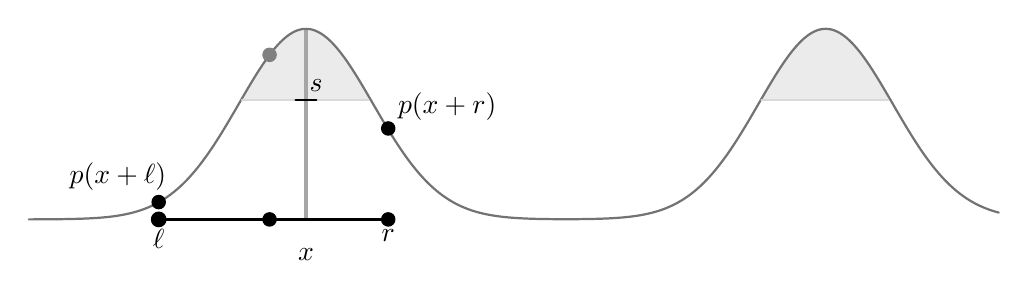
\begin{tikzpicture}[scale=1.1, line cap=round, line join=round]

    % Shaded slice region 1
    \fill[black!8, domain=2.26:3.72, samples=200]
    plot (\x, {
        2.2*exp(-((\x-3.0)^2)/1.2)
    })
    --
    (3.72,1.38)
    --
    (2.26,1.38)
    -- cycle;

    % Shaded slice region 2
    \fill[black!8, domain=8.26:9.72, samples=200]
    plot (\x, {
        2.2*exp(-((\x-9.0)^2)/1.2)
    })
    --
    (9.72,1.38)
    --
    (8.26,1.38)
    -- cycle;

    % Vertical line at t=0
    \draw[very thick, black!35] (3.0,0) -- (3.0,2.19);
    
    % Density curve
    \draw[thick, black!55, smooth, samples=200, domain=-0.2:11.0]
        plot (\x, {
            2.2*exp(-((\x-3.0)^2)/1.2)
          + 2.2*exp(-((\x-9.0)^2)/1.2)
        });

    % Horizontal slice level
    \draw[very thick] (1.3,0) -- (3.95,0);

    % Short horizontal guide to s
    \draw[thick, black!15] (2.26,1.38) -- (3.72,1.38);
    \draw[thick, black!15] (8.26,1.38) -- (9.72,1.38);

    % Mark s on vertical line
    \draw[thick] (2.88,1.38) -- (3.12,1.38);
    \node[right] at (2.93,1.55) {$s$};

    % Labels for interval endpoints and t=0
    \node[below] at (1.3,0) {$\ell$};
    \node[below] at (3.95,0) {$r$};
    \node[below] at (3.0,-0.22) {$\boldsymbol{x}$};

    % p(l) and p(r) labels
    \node[left] at (1.5,0.5) {$p(\boldsymbol{x} + \ell)$};
    \node[right] at (3.95,1.3) {$p(\boldsymbol{x} + r)$};

    % Endpoint markers (filled circles)
    \filldraw[black] (1.3,0) circle (2.4pt);
    % \filldraw[black] (5.3,0) circle (2.4pt);

    % Interior rejected/proposed points on baseline
    \filldraw[black] (2.58,0) circle (2.2pt);
    \filldraw[black] (3.95,0) circle (2.2pt);

    % Points on the upper contour
    \filldraw[black] (1.3,0.2) circle (2.2pt);
    \filldraw[gray] (2.58,1.9) circle (2.2pt);
    \filldraw[black] (3.95,1.05) circle (2.2pt);

    \end{tikzpicture}

    \caption{Visualization of the step-out procedure. The shaded gray area shows the region $L(s)$, the step-out procedure took two steps to the left and one step to the right until stoppage. For a multimodal distribution the step-out procedure misses the second mode if the step-size $w$ is not large enough.}
    \label{fig:stepout}
\end{figure}



\paragraph{Shrinkage procedure} 
Given the interval $(l,r)$ the shrinkage procedure draws a valid proposal by iteratively reducing the interval until a proposal falls in the intersection with the slice $L(s)$. We follow the presentation of \citet{durmus2026geodesic} which differs slightly from the original formulation of \citet{Neal2003}. The procedure works as follows. Let $J = (\ell,r)$ and sample $a\sim \mathrm{Unif}(J)$, if $\gamma_x(a)\in L(s)$ the proposal is $\gamma_x(a) = x+a$. If not, sample  $b\sim \mathrm{Unif}(J)$, if $\gamma_x(b)\in L(s)$ the proposal is $\gamma_x(b) = x+b$. Otherwise shrink the interval $J$ by
\begin{itemize}    
    \item Update $J$ as
    \begin{equation*}
        J =
        \begin{cases} 
        % J\cap(a \wedge b, a \vee b), & \text{if } 0 \in J, \\
        % J \setminus (a \wedge b, a\vee b), & \text{if } 0 \notin J.
        J \cap \bigl(\min(a,b), \max(a,b)\bigr), & \text{if } 0 \in J, \\
        J \setminus \bigl(\min(a,b), \max(a,b)\bigr), & \text{if } 0 \notin J.
        \end{cases}        
    \end{equation*}    
    \item Set $a\gets b$ and  sample $b\sim \mathrm{Unif}(J)$.  
    \item Repeat until $\gamma_x(b) \in L(s)$.
\end{itemize}


\paragraph{Hit-and-Run slice sampling} 
There are multiple ways of extending slice sampling to multivariate distributions \citep{Neal2003, Murray2010}. Here we consider the Hit-and-Run \citep{Belisle1993} extension which is relevant for our method. Denote the unit sphere by $\mathbb{S}^{D-1} := \{\boldsymbol{v} \in \mathbb{R}^D : \norm{\boldsymbol{v}}^2 =1\}$. Given current position $\boldsymbol{x}\in \mathbb{R}^{D}$:
\begin{itemize}
    \item Sample direction $\boldsymbol{v}\sim \mathrm{Unif}(\mathbb{S}^{D-1}(\boldsymbol{x}))$.
    \item Define $\gamma_{(\boldsymbol{x},\boldsymbol{v})}(t)  = \boldsymbol{x} + t \boldsymbol{v}$ and apply one dimensional slice sampling on $t \mapsto \gamma_{(\boldsymbol{x},\boldsymbol{v})}(t)$.
\end{itemize}
Since the straight line $\gamma_{(\boldsymbol{x},\boldsymbol{v})}(t)$ defines a univariate distribution, slice sampling is directly applicable. Concretely, one transition of hit-and-run slice sampling consists of the following steps: Sample $s\sim \mathrm{Unif}(0, p(\boldsymbol{x}))$, then the step-out procedure returns the interval 
$$\ell,r = \text{Step-out}_{w,m}(s, \gamma_{(\boldsymbol{x},\boldsymbol{v})}),$$
and the shrinkage procedure gives the proposal
$$t^* = \text{Shrink}_{\ell,r}(s, \gamma_{(\boldsymbol{x},\boldsymbol{v})}).$$ 
Finally the new sample after one step of the algorithm is $\boldsymbol{x}' = \gamma_{(\boldsymbol{x},\boldsymbol{v})}(t^*)$. This allows sampling from target distributions defined on $\mathbb{R}^D$. See Figure~\ref{fig:hitandrun} for a visualization of the hit-and-run procedure.
\begin{figure}
    \centering
    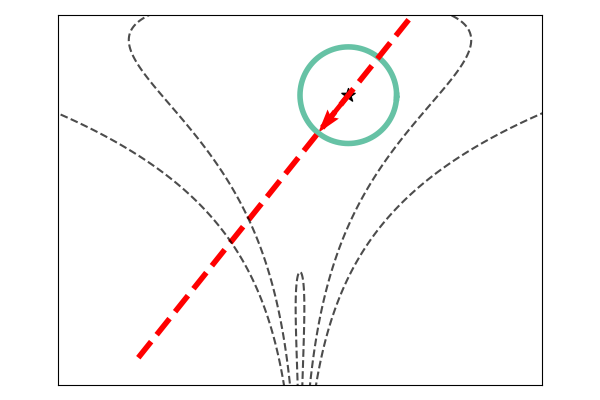
\includegraphics[width=0.49\linewidth]{figs/paper2/hitandrun/geodesic_balls_euclidean_hitandrun.png}
    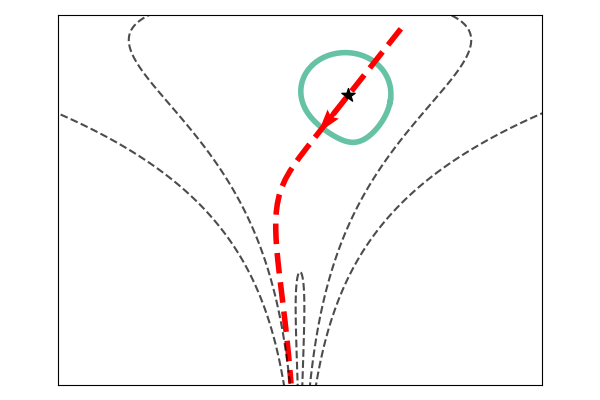
\includegraphics[width=0.49\linewidth]{figs/paper2/hitandrun/geodesic_balls_monge_hitandrun.png}
    \caption{Visualization of the hit-and-run procedure. Left:  A velocity uniformly sampled uniformly on $\mathbb{S}^{D-1}$ (blue) and the resulting straight line (dotted red line). Right:  A velocity sampled uniformly from $\{\boldsymbol{v}: \|\boldsymbol{v}\|^2_{\mathbf{G}(\boldsymbol{x})} =1\}$ and the geodesic captures better the geometry of the target (dotted red line).}
    \label{fig:hitandrun}
\end{figure}

\subsection{Geometric MCMC}
By geometric MCMC we refer to MCMC methods that incorporate a Riemannian tensor in the sampling method.
The main benefit is the adaptation to local curvature, but the introduction of a non-flat geometry results in higher computational cost. 
Recall that 
\begin{equation*}
 \mathbf{G}(\cdot):\mathbb{R}^D\to \mathbb{R}^D\times \mathbb{R}^D,   
\end{equation*}
is the matrix  that holds the components of a metric tensor (see Section~\ref{sec:riemannian_background}). 
Next we describe some geometric MCMC methods and their computational cost.

\paragraph{Riemannian manifold Hamiltonian Monte Carlo (RMHMC) }
The seminal work of \citet{Girolami2011} extended two gradient-based sampling methods,  Metropolis-adjusted Langevin algorithm (MALA) and Hamiltonian Monte Carlo (HMC) from Euclidean space to a Riemannian setting. Here we only describe the HMC extension. Both HMC and RMHMC introduce an auxiliary momentum $\boldsymbol{p}\in\mathbb{R}^D$ and model a system of ordinary differential equations (ODEs). The goal is that the solution to the ODEs generates samples that are further away from the initial state reducing sample correlation. The Hamiltonian equation is
\begin{equation*}
    \mathcal{H}(\boldsymbol{x},\boldsymbol{p})
    =
    \phi(\boldsymbol{x})
    +
    \frac{1}{2}\boldsymbol{p}^{\top}\mathbf{G}(\boldsymbol{x})^{-1}\boldsymbol{p},
\end{equation*}
where $\phi(\boldsymbol{x})=-\ell(\boldsymbol{x})+ \frac{1}{2}\log\det \mathbf{G}(\boldsymbol{x})$. The dynamics are given by the differential equations obtained from differentiation of $\mathcal{H}(\boldsymbol{x},\boldsymbol{p})$
\begin{equation}
    \dot{\boldsymbol{x}} = \mathbf{G}(\boldsymbol{x})^{-1}\boldsymbol{p},
    \quad
    \dot{\boldsymbol{p}} = - \nabla_{\boldsymbol{x}} \mathcal{H}(\boldsymbol{x},\boldsymbol{p}).
    \label{eq:rmhmc}
\end{equation}
The numerical integration of Equation~\ref{eq:rmhmc} relies on fixed point iteration \citep{Girolami2011}. Each step iterates until a specified tolerance is reached to generate a proposal, increasing the runtime. With a full rank metric tensor the resulting computations are of order $\mathcal{O}(D^3)$ at each iteration,  which limits its scalability to high dimensional problems.

\paragraph{Lagrangian dynamical Monte Carlo (LMC) }
\citet{Lan2015} expressed the Hamiltonian equations in terms of velocity instead of momentum through a change of variables  $\boldsymbol{v}=\mathbf{G}(\boldsymbol{x})^{-1}\boldsymbol{p}$, and the system dynamics become
\begin{equation}
    \dot{\boldsymbol{x}} = \boldsymbol{v},
    \quad
    \dot{\boldsymbol{v}} = -\boldsymbol{\eta}(\boldsymbol{x},\boldsymbol{v}) - \mathbf{G}(\boldsymbol{x})^{-1}\nabla_{\boldsymbol{x}}\phi(\boldsymbol{x}),
    \label{eqsLMC}
\end{equation}
where $[\boldsymbol{\eta}(\boldsymbol{x},\boldsymbol{v})]_k=\sum_{i,j}\Gamma^k_{ij}(\boldsymbol{x})\,v_i v_j$, and the Christoffel symbols $\Gamma_{ij}^k$ are defined in Equation~\ref{eq:christoffel_symbols}. 
The authors proposed a numerical integrator that is explicit and does not rely on fixed point iterations, improving the running time over RMHMC. Each step still computes inverses of the metric tensor and is $\mathcal{O}(D^3)$ in complexity which again limits its scalability to higher dimensions. One way of reducing the complexity of the numerical integrators is to use metrics with closed form inverses and determinants \citep{Hartmann2022}. Some metric choices are presented in Chapter~\ref{ch:mcmc}.
Additionally, the numerical integrator introduces two hyperparameters, the step-size and the number of steps, with several strategies available for selecting a value. \citet{williams2024geometric} discuss the choice of metric, numerical integrator, and hyperparameter adaptation in RMHMC and LMC. 

\section{Modeling discrete data} \label{sec:discrete_data}

We study two problems: discrete-data generation and classification. For generative modeling we consider flow matching and Riemannian flow matching, while for classification we use Gaussian processes. 
We first review flow-based models and a Riemannian flow matching approach used for generative modeling of discrete data, and then we review Gaussian process classification. Both approaches model a continuous latent process that produces discrete outputs via an $\arg\max$ operation. In the first case the latent model is flow based, and in the second it is a Gaussian process.  

\subsection{Discrete data generation}


We first discuss two continuous generative models that are building blocks: conditional flow matching which operates in the Euclidean space, then Riemannian flow matching which operates on manifolds. Then we present a method for discrete data generation which operates on the simplex and uses the Fisher geometry. 

\paragraph{Conditional flow matching (CFM)}
Conditional flow matching is a generative model for continuous data in the Euclidean space \citep{Albergo2023,Lipman2023,liu2023flow}. 
For $\boldsymbol{x}\in \mathbb{R}^D$, the model defines a vector field
$\boldsymbol{u}_t:\mathbb{R}^D\times[0,1]\to\mathbb{R}^D$,
which evolves data according to 
\begin{equation}
    \frac{d\boldsymbol{x}_t}{dt}=\boldsymbol{u}_t(\boldsymbol{x}_t), \qquad \boldsymbol{x}_t\sim p_t,
    \label{eq:cfm_ode}
\end{equation}
where the initial condition is a simple base distribution $p_0$ that allows direct generation of samples and density evaluation, and the final condition is the data distribution $p_1=p_{\mathrm{data}}$. The marginal probability path $\{p_t\}_{t\in[0,1]}$ is linked to $\boldsymbol{u}_t$ by the continuity equation, this gives the instantaneous change of variable formula, which is useful for computing log-densities
\begin{equation*}
    \dv[]{\log p_t(x_t)}{t} = - \div(u_t(x_t)).
\end{equation*}
In practice $\boldsymbol{u}_t$ is not available, instead a parametric model (usually a neural network) $\boldsymbol{v}_t^\theta$ is fit to the conditional vector fields $\boldsymbol{u}_t(\boldsymbol{x}_t\mid\boldsymbol{x}_0,\boldsymbol{x}_1)$, the resulting objective is
\begin{equation}
\mathcal{L}_{\mathrm{CFM}}(\theta)
= \mathbb{E}_{\substack{t\sim \mathrm{Unif}(0,1) \\ \boldsymbol{x}_0,\boldsymbol{x}_1\sim\pi(\boldsymbol{x}_0,\boldsymbol{x}_1)}}
  \left\| \boldsymbol{v}^\theta_t\big(\boldsymbol{x}_t\big) - \boldsymbol{u}_t(\boldsymbol{x}_t|\boldsymbol{x}_0,\boldsymbol{x}_1) \right\|_2^2, \label{eq:cfm_loss}
\end{equation}
 where $\pi$ is any coupling with marginals $p_0$ and $p_1$. \citet{Lipman2023} show that this conditional objective equals up to a constant, the objective for estimating $\boldsymbol{u}_t(\boldsymbol{x}_t)$ directly. Therefore, $\boldsymbol{v}^\theta_t\big(\boldsymbol{x}_t\big)$ is used in  Equation~\ref{eq:cfm_ode} to generate new data. The velocity field depends on the interpolation path between $\boldsymbol{x}_0$ and $\boldsymbol{x}_1$.  A common choice is the linear interpolation $\boldsymbol{x}_t=(1-t)\boldsymbol{x}_0+t\boldsymbol{x}_1$
which yields the constant conditional velocity
\[
\boldsymbol{u}_t(\boldsymbol{x}_t\mid\boldsymbol{x}_0,\boldsymbol{x}_1)=\dot{\boldsymbol{x}}_t=\boldsymbol{x}_1-\boldsymbol{x}_0.
\]
Two common options for the joint density of $\boldsymbol{x}_0,\boldsymbol{x}_1$ are the independent coupling $\pi(\boldsymbol{x}_0,\boldsymbol{x}_1)=p_0(\boldsymbol{x}_0)p_1(\boldsymbol{x}_1)$ and optimal-transport coupling.
The optimal transport coupling is approximated with mini-batch optimal transport and typically improves optimization stability while reducing the number of function evaluations needed at sampling time \citep{Tong2024}.


\paragraph{Riemannian conditional flow matching (RCFM)}
Conditional flow matching can be extended from Euclidean space to a Riemannian manifold $(\mathcal{M}, \mathbf{G})$ \citep{Chen2024}. 
Instead of a vector field in the Euclidean space $\mathbb{R}^D$, the vector field is defined on the tangent space of the manifold $\boldsymbol{u}_t(\boldsymbol{x})\in T_{\boldsymbol{x}}\mathcal{M}$. The resulting dynamics on the manifold are
\[
\frac{d\boldsymbol{x}_t}{dt} = \boldsymbol{u}_t(\boldsymbol{x}_t), \qquad \boldsymbol{x}_t\sim p_t,
\]
where the initial condition is a simple base distribution defined over $\mathcal{M}$.
The marginal probability paths are generated from $\boldsymbol{u}_t$ by the Riemannian version of the instantaneous change of variables 
\begin{equation*}
    \dv[]{\log p_t(\boldsymbol{x}_t)}{t} = - \operatorname{div}_{\mathbf{G}}(\boldsymbol{u}_t(\boldsymbol{x}_t)), 
\end{equation*}
where $\operatorname{div}_\mathbf{G}$ is the Riemannian divergence \citep{Lee2018}. Similarly to the Euclidean case, $\boldsymbol{u}_t$ is not available, but we can train the parametric model $\boldsymbol{v}_t^\theta$ using the conditional objective 
\begin{equation*}
\mathbb{E}_{\substack{t\sim \mathrm{Unif}(0,1) \\ \boldsymbol{x}_0,\boldsymbol{x}_1\sim\pi(\boldsymbol{x}_0,\boldsymbol{x}_1)} }
\left\|\boldsymbol{v}_t^\theta(\boldsymbol{x}_t){-}\boldsymbol{u}_t(\boldsymbol{x}_t\mid \boldsymbol{x}_0,\boldsymbol{x}_1)\right\|^2_{\mathbf{G}(\boldsymbol{x}_t)}.
\end{equation*}
Here $\| \boldsymbol{v}  \|_{\mathbf{G}(\boldsymbol{x}_t)} := \sqrt{\boldsymbol{v}^\top \mathbf{G}(\boldsymbol{x}_t)\boldsymbol{v} } $ is the norm induced by the metric $\mathbf{G}$ at $\boldsymbol{x}_t$. The tangent velocity field depends on the interpolation, a standard choice is the geodesic which connects $\boldsymbol{x}_0$ and  $\boldsymbol{x}_1$, defined by  $\boldsymbol{x}_t = \operatorname{Exp}_{\boldsymbol{x}_0}( t \boldsymbol{v})$ and $\boldsymbol{v} = \operatorname{Log}_{\boldsymbol{x}_0}(\boldsymbol{x}_1)$. This choice gives the conditional target velocity
\[
\boldsymbol{u}_t(\boldsymbol{x}_t\mid\boldsymbol{x}_0,\boldsymbol{x}_1)
=\frac{\operatorname{Log}_{\boldsymbol{x}_t}(\boldsymbol{x}_1)}{1-t}, \quad \boldsymbol{x}_t = \operatorname{Exp}_{\boldsymbol{x}_0}( t \operatorname{Log}_{\boldsymbol{x}_0}(\boldsymbol{x}_1)).
\]
When $\mathcal{M}=\mathbb{R}^D$ with the Euclidean metric, these expressions reduce to standard CFM.
If the manifold does not have closed form geodesics and logarithm map, then training and inference rely on approximations of these quantities. As in CFM, $\pi(\boldsymbol{x}_0,\boldsymbol{x}_1)$ can be the independent coupling or the optimal transport coupling. On the manifold, the geodesic distance of two points is the length of the geodesic between them, mini-batch optimal transport computes the transport cost with respect to this distance. 



\paragraph{Discrete data generation with the Fisher geometry}
\citet{Cheng2024} and \citet{Davis2024} introduced Categorical Flow Matching on Statistical Manifolds (SFM), a special case of Riemannian flow matching for discrete data. In this model the manifold is the simplex and the metric is the Fisher information metric. In practice, the flow could be modeled directly on the simplex, but computations become unstable near the boundaries, where discrete observations lie. SFM therefore models  Riemannian flow matching on the sphere instead. We first introduce the simplex geometry with the Fisher metric, then establish the isomorphism with the sphere, and finally specify the training and sampling procedures. 

Let $K$ be the number of categories and $D:=K-1$ the latent dimension. Consider the simplex $\Delta^{D}:=\{\boldsymbol{x}\in\mathbb{R}_{\ge 0}^{K}:\;\sum_{k=1}^{K}x_k=1\}$, and endow the space with the Fisher information metric of the categorical distribution \citep{Miyamoto2024}
\begin{equation*}
 \mathbf{G}_F(\boldsymbol{x}) = \mathrm{diag}\left(\frac{1}{\boldsymbol{x}_{1:D}}\right) + \frac{1}{x_K} \mathbf{1}\mathbf{1}^\top.
\end{equation*}
Under the Fisher metric, the space has the inner product for $\boldsymbol{u},\boldsymbol{v}\in T_{\boldsymbol{x}}\Delta^D$,
\begin{align*}
    \inp{\boldsymbol{u}}{\boldsymbol{v}}_{G_F(\boldsymbol{x})} = \sum_{i=1}^D \frac{u_iv_i}{x_i} + \frac{( \sum_{i=1}^D u_i)( \sum_{i=1}^D v_i)}{x_K}  = \sum_{i=1}^K \frac{u_i v_i}{x_i}.
\end{align*}
The last equality uses the tangent space constraint in the ambient space $T_{\boldsymbol{x}}\Delta^D = \{\boldsymbol{u}\in\mathbb{R}^K: \sum_{i=1}^K u_i = 0\}$ so $u_K = -\sum_{i=1}^D u_i $.
Note that the inner product is only defined on $\mathring{\Delta}^D$, since it is undefined on the boundary. The bijection between the simplex and the positive orthant of the sphere, together with its inverse, is given by
\begin{equation}
\begin{aligned}
\varphi: \Delta^{D} \to \mathbb{S}_+^{D}, \quad
&\boldsymbol{x}\mapsto \boldsymbol{z} = \sqrt{\boldsymbol{x}},\quad \text{and}\\
\varphi^{-1}: \mathbb{S}_+^{D} \to \Delta^{D}, \quad
&\boldsymbol{z} \mapsto \boldsymbol{x} = \boldsymbol{z}^2.
\end{aligned}
\label{eq:bij_sfm}
\end{equation}
$\mathbb{S}_{+}^{D} := \{ \boldsymbol{z} \in \mathbb{R}_{\ge 0}^{K} : \sum_{k=1}^{K} z_k^2 = 1 \}$, and the square root and squaring operations are applied component wise. 
This bijection (illustrated in Figure~\ref{fig:simplex-sphere-map}) is in fact an isomorphism between $(\Delta^D  , \mathbf{G}_F)$ and $(\mathbb{S}_{+}^{D}, \mathbf{G})$, where $\mathbf{G}$ is the canonical metric on the sphere \citep{Miyamoto2024}. The sphere is embedded in $\mathbb{R}^K$, and it inherits the ambient space inner product restricted to the tangent space, for $\boldsymbol{u},\boldsymbol{v}\in T_{\boldsymbol{z}} \mathbb{S}_{+}^{D}$,
\begin{equation*}
    \inp{\boldsymbol{u}}{\boldsymbol{v}}_G = \inp{\boldsymbol{u}}{\boldsymbol{v}}_2 = \sum_{i=1}^K u_i v_i.
\end{equation*} 
The geodesics in the sphere are the outer rings, the exponential and  logarithm map are
\begin{equation}
\begin{aligned}
\operatorname{Exp}_{\boldsymbol{z}}( t \boldsymbol{v}) 
&= \cos\!\bigl(t\|\boldsymbol{v}\|_2\bigr)\boldsymbol{z}
+ \sin\!\bigl(t\|\boldsymbol{v}\|_2\bigr)\frac{\boldsymbol{v}}{\|\boldsymbol{v}\|_2}, \text{ and}\\
\operatorname{Log}_{\boldsymbol{z}}(\boldsymbol{z}')
&= \frac{\theta}{\sin\theta}\Bigl(\boldsymbol{z}' - \cos(\theta)\boldsymbol{z}\Bigr), \text{ where }
\theta = \arccos\!\bigl(\inp{\boldsymbol{z}}{\boldsymbol{z}'}\bigr).
\end{aligned}
\label{eq:geo_sphere}
\end{equation}
\begin{figure}
  \centering
\begin{tikzpicture}
  \def\r{2}

  \begin{scope}
    \coordinate (O)  at (0,0);
    \coordinate (X1) at ({-\r/sqrt(10)}, {-\r/sqrt(10)});
    \coordinate (X2) at ({\r},0);
    \coordinate (X3) at (0,{\r});

    % Straight edges for the simplex
    \draw[line width=1.4pt] (X1) -- (X2);
    \draw[line width=1.4pt] (X1) -- (X3);
    \draw[line width=1.4pt] (X2) -- (X3);

    % Axes
    \draw[->] (O) -- ({-1.15*\r/sqrt(10)}, {-1.15*\r/sqrt(10)}) node[below] {$x_1$};
    \draw[->] (O) -- ({1.15*\r}, 0) node[right] {$x_2$};
    \draw[->] (O) -- (0, {1.15*\r}) node[above] {$x_3$};
    \node[anchor=north west] at (-1.5, 2.5) {\Large $\Delta^2$};

    \node[
      star,
      star points=5,
      star point ratio=2.25,
      fill=green!50!black,
      draw=green!50!black,
      minimum size=9pt,
      inner sep=0pt
    ] at (0.5,0.5) {};
    \node[above right, text=green!50!black] at (0.5,0.5) {$x$};
  \end{scope}

  \draw[<->, line width=2pt] (2.9,1.1) -- (5.3,1.1)
    node[midway, above, font=\Large] {$\varphi$}
    node[midway, below, font=\Large] {$\varphi^{-1}$};

  \begin{scope}[xshift=6.5cm]
    % Axes
    \draw[->] (0,0) -- ({-1.15*\r/sqrt(10)}, {-1.15*\r/sqrt(10)}) node[below] {$z_1$};
    \draw[->] (0,0) -- ({1.15*\r}, 0) node[right] {$z_2$};
    \draw[->] (0,0) -- (0, {1.15*\r}) node[above] {$z_3$};
    \node[anchor=north west] at (-1.5, 2.5) {\Large $\mathbb{S}_+^2$};

    % Arcs for the spherical section
    \draw[line width=1.4pt] (\r, 0) arc [start angle=0, end angle=90, x radius=\r, y radius=\r];
    \draw[line width=1.4pt] (0, \r) arc [start angle=90, end angle=198, x radius=\r/3, y radius=\r];
    \draw[line width=1.4pt] ({-\r/sqrt(10)}, {-\r/sqrt(10)}) arc [start angle=-108, end angle=0, x radius=\r, y radius=\r/3];
    
    \node[
      star,
      star points=5,
      star point ratio=2.25,
      fill=green!50!black,
      draw=green!50!black,
      minimum size=9pt,
      inner sep=0pt
    ] at (0.7,0.7) {};
    \node[above right, text=green!50!black] at (0.7,0.7) {$\varphi(x)$};
  \end{scope}
\end{tikzpicture}
  \caption{Visual illustration of the simplex-to-sphere map.}
  \label{fig:simplex-sphere-map}
\end{figure}


\begin{proposition}[Isometry, \citep{amari2000methods, Miyamoto2024}]
\label{prop:isomorphism_fisher}
The diffeomorphism in Equation~\ref{eq:bij_sfm} is an isomorphism between $(\Delta^D  , \mathbf{G}_F)$  and $(\mathbb{S}_{+}^{D}, \mathbf{G})$ up to a factor of $\frac{1}{4}$.
\end{proposition}
\begin{proof}
    The proof consists of showing
    $
    \frac{1}{4}\inp{\boldsymbol{u}}{\boldsymbol{v}}_{\mathbf{G}_F(\boldsymbol{x})}
    =
    \inp{\mathrm{d}\varphi_{\boldsymbol{x}}(\boldsymbol{u})}{\mathrm{d}\varphi_{\boldsymbol{x}}(\boldsymbol{v})}
    $
    for all $\boldsymbol{x}\in \Delta^D$ and $\boldsymbol{u},\boldsymbol{v}\in T_{\boldsymbol{x}}\Delta^D$, where $\mathrm{d}\varphi_{\boldsymbol{x}}(\boldsymbol{v})$ denotes the differential of $\varphi$ at $\boldsymbol{x}$ applied to the tangent vector $\boldsymbol{v}$. Since $\mathbb{S}_{+}^{D}$ is embedded in $\mathbb{R}^K$, we use the ambient Euclidean inner product
    \begin{align*}
        \inp{\mathrm{d}\varphi_{\boldsymbol{x}}(\boldsymbol{u})}{\mathrm{d}\varphi_{\boldsymbol{x}}(\boldsymbol{v})}
        &=
        \inp{\eval{\dv{}{t}\varphi(\boldsymbol{x}+t\boldsymbol{u})}_{t=0}}
            {\eval{\dv{}{t}\varphi(\boldsymbol{x}+t\boldsymbol{v})}_{t=0}} \\
        &=
        \inp{ \left(
\frac{u_1}{2\sqrt{x_1}},\dots,\frac{u_K}{2\sqrt{x_K}}
\right) }
            {\left(
\frac{v_1}{2\sqrt{x_1}},\dots,\frac{v_K}{2\sqrt{x_K}}
\right)} \\
        &= \frac{1}{4}\sum_{i=1}^K \frac{u_i v_i}{x_i}
        = \frac{1}{4}\inp{\boldsymbol{u}}{\boldsymbol{v}}_{\mathbf{G}_F(\boldsymbol{x})}.
    \end{align*}
\end{proof}
Based on the isomorphism (Proposition~\ref{prop:isomorphism_fisher}), the exponential map in $(\Delta^D  , \mathbf{G}_F)$ is 
\begin{align*}
\operatorname{Exp}_{\boldsymbol{x}}( t \boldsymbol{v})  &= \varphi^{-1}\big(\mathrm{Exp}_{\sqrt{x}}(d\varphi_x(v))\big) \\
& = \left(
\cos\!\left(\frac{t\|\boldsymbol{v}\|_{\mathbf{G}_F(\boldsymbol{x})}}{2}\right)\sqrt{\boldsymbol{x}}
+
\sin\!\left(\frac{t\|\boldsymbol{v}\|_{\mathbf{G}_F(\boldsymbol{x})}}{2}\right)
\frac{\boldsymbol{v}}{\|\boldsymbol{v}\|_{\mathbf{G}_F(\boldsymbol{x})}\sqrt{\boldsymbol{x}}}
\right)^2.
\label{eq:geo_simplex}
\end{align*}
Note that $\|\cdot \|_{\mathbf{G}_F}$ and $\tfrac{1}{\sqrt{\boldsymbol{x}}}$ explode when $\boldsymbol{x}$ approaches $\partial \Delta^D$ which makes it unstable, to address this  \citet{Cheng2024} and \cite{Davis2024} proposed modeling directly in the sphere. The approach first transforms the training data to the sphere with $\varphi$, and then fits the flow's parameters with RCFM on this space (Algorithm~\ref{alg:train_sfm}). New data is sampled by numerical integration of the learned velocity field, and the final point is mapped to the simplex with $\varphi^{-1}$ (Algorithm~\ref{alg:sample_sfm}).

\begin{algorithm}
\caption{Training of SFM.}
\label{alg:train_sfm}
\begin{algorithmic}[1]
\Require Data $\boldsymbol{x}\!\in\!\Delta^{D}$, bijection $\varphi$, base $p_0$ (e.g. $\varphi_\sharp \mathrm{Unif}(\Delta^D)$), 
coupling $\pi$ (indep. or minibatch OT)
\For{each mini-batch}    
  \State $\boldsymbol{z}_1 \gets \varphi({\boldsymbol{x}})$ \Comment{Map to the sphere.}
  \State Sample $\boldsymbol{z}_0 \sim p_0$; pair $(\boldsymbol{z}_0,\boldsymbol{z}_1)$ via $\pi$
  \State Sample $t\sim \mathrm{Unif}(0,1)$
  \State $\boldsymbol{z}_t\!\gets\!\operatorname{Exp}_{\boldsymbol{z}_0}( t \operatorname{Log}_{\boldsymbol{z}_0}(\boldsymbol{z}_1))$, \;
         $\boldsymbol{u}_t\!\gets\!{\operatorname{Log}_{\boldsymbol{z}_t}(\boldsymbol{z}_1)}/({1-t})$
  \State Update $\theta$ by 
  $\min \|\boldsymbol{v}_t^\theta(\boldsymbol{z}_t)-\boldsymbol{u}_t\|_{\mathbf{G}(\boldsymbol{z}_t)}^2$ \; 
\EndFor
\end{algorithmic}
\end{algorithm}

\begin{algorithm}[t]
\caption{Sampling with SFM.}
\label{alg:sample_sfm}
\begin{algorithmic}[1]
\Require Learned $\boldsymbol{v}_\theta$, bijection $\varphi$, base $p_0$
\State Sample $\boldsymbol{z}_0 \sim p_0$ 
\State Solve ODE: 
$\tfrac{d\boldsymbol{z}_t}{dt} = \boldsymbol{v}_\theta(\boldsymbol{z}_t,t), \; t\!\in[0,1], \boldsymbol{z}_t\in \mathbb{S}^D$
\State $\hat{\boldsymbol{x}} \gets \varphi^{-1}(\boldsymbol{z}_1)$
\end{algorithmic}
\end{algorithm}

\subsection{Gaussian processes for classification} \label{sec:gp}

We first briefly introduce Gaussian processes.  We then describe two sparse formulations based on inducing points. Finally we present Dirichlet-based Gaussian process classification, which uses label smoothing and a distributional approximation to turn classification into Gaussian process regression in the latent space. These topics provide together the background for Paper~IV.

\paragraph{Gaussian process}

A Gaussian process (GP) \citep{williams2006gaussian} defines a distribution over functions such that any finite collection of function values is jointly Gaussian. It provides a flexible prior together with uncertainty quantification. Given a finite set of inputs $\boldsymbol{x}_1,\ldots,\boldsymbol{x}_N\in\mathbb{R}^P$ the distribution over values $(f(\boldsymbol{x}_1), .., f(\boldsymbol{x}_N))$ is multivariate Gaussian, where the mean is specified by a mean function $m:\mathbb{R}^P\to\mathbb{R}$ and the covariance between any pair of points by a kernel $K_\theta:\mathbb{R}^P\times\mathbb{R}^P\to\mathbb{R}$ dependent on hyperparameters $\theta$. The GP prior is written  as 
\[
f \sim \mathcal{GP}\!\bigl(m(\cdot),\,K_{\theta}(\cdot,\cdot)\bigr).
\]
Consider a supervised regression problem where the data is denoted $\mathcal{D}:=\{(\boldsymbol{x}_n,\boldsymbol{z}_n)\}_{n=1}^N$ for $\boldsymbol{x}_n\in\mathbb{R}^P$ and $\boldsymbol{z}_n\in\mathbb{R}^D$. 
In practice, the responses are usually centered by subtracting the empirical mean, and the mean function is set to zero. 
The kernel function imposes assumptions on the correlation of the latent functions and on the behavior of the function space. For example, different kernels can model periodic behaviors, or be translation invariant. In this work we consider the radial basis function kernel
\[
K_{\theta}(\boldsymbol{x},\boldsymbol{x}')
=
\sigma_f^2\exp\!\left(-\frac{\|\boldsymbol{x}-\boldsymbol{x}'\|_2^2}{2\ell^2}\right),
\qquad
\theta=(\sigma_f^2,\ell),
\]
where $\sigma_f^2$ controls the variance and $\ell$ is the length scale which controls how fast the dependency between $\boldsymbol{x}$ and $\boldsymbol{x}'$ decays. This kernel gives smooth latent functions. 

Although it is possible to introduce dependency among dimensions \citep{goulard1992linear}, in this thesis, we model $D$ independent GPs (one per dimension) denoted $\mathbf{f} = (f^{(1)}, .., f^{(D)})$, and the same kernel is shared across $D$-dimensions. 
Given a  GP prior assume the noisy Gaussian likelihood
 \[
\boldsymbol z_n\mid \mathbf f(\boldsymbol{x}_n) \sim \mathcal N\!\bigl(\mathbf f(\boldsymbol{x}_n),\,\sigma^2\mathbf I_D\bigr).
\]
Let $\boldsymbol{x}_*\in\mathbb{R}^P$ be a test input and denote the vector of responses $\boldsymbol{z}^{(d)} := \bigl(z_1^{(d)},\ldots,z_N^{(d)}\bigr)^\top \in \mathbb{R}^N$ for $d=1,..,D$. The joint distribution of $\boldsymbol{z}^{(d)}$ and $f^{(d)}(\boldsymbol{x}_*)$ is
\begin{equation*}
\begin{bmatrix}
\boldsymbol{z}^{(d)} \\
f^{(d)}(\boldsymbol{x}_*)
\end{bmatrix}
\sim
\mathcal{N}\!\left(
\boldsymbol{0},
\begin{bmatrix}
\mathbf{K}_N + \sigma^2 \mathbf{I}_N & \mathbf{k}_* \\
\mathbf{k}_*^\top & k_{**}
\end{bmatrix}
\right),
\end{equation*}
where the covariance entries are given by
$[\mathbf{K}_N]_{ij} = k_\theta(\boldsymbol{x}_i,\boldsymbol{x}_j)$, $[\mathbf{k}_*]_i = k_\theta(\boldsymbol{x}_i,\boldsymbol{x}_*)$, and $k_{**} = k_\theta(\boldsymbol{x}_*,\boldsymbol{x}_*)$.
The standard predictive posterior is obtained by conditioning on the observations  \citep{williams2006gaussian}, it is distributed as
$f^{(d)}(\boldsymbol{x}_*) \mid \boldsymbol{z}^{(d)}
\sim
\mathcal{N}\!\bigl(\mu_*^{(d)},\,\sigma_*^2\bigr)$ with mean and covariance
\begin{equation}
\begin{aligned}
\mu_*^{(d)} &:=\mathbf k_*^\top(\mathbf{K}_{N}+\sigma^2\mathbf I_N)^{-1}\boldsymbol z^{(d)}, \text{ and}\\
\sigma_*^2 &:= k_{**}-\mathbf k_*^\top(\mathbf{K}_{N}+\sigma^2\mathbf I_N)^{-1}\mathbf k_*.
\end{aligned}
\label{eq:gp_posterior}
\end{equation}
We can write it compactly in a single expression
\begin{equation*}
 \mathbf f_*\mid\mathcal D\sim\mathcal N(\boldsymbol\mu_*,\boldsymbol\Sigma_*),   
\end{equation*}
with $\boldsymbol\mu_*:=(\mu_*^{(1)},\ldots,\mu_*^{(D)})^\top$ and $\boldsymbol\Sigma_*:=\sigma_*^2\mathbf I_D$. The marginal log-likelihood is used to learn the kernel hyperparameters. Since the likelihood is Gaussian and the output dimensions are assumed independent, it takes the form 
\begin{equation}
\log p\bigl(\boldsymbol{z} \mid \theta\bigr)
= -\tfrac12\sum_{d=1}^D \|\boldsymbol z^{(d)}\|^2_{(\mathbf{K}_{N}+\sigma^2\mathbf I_N)^{-1}}
- \tfrac{D}{2}\log\lvert\mathbf{K}_{N}+\sigma^2\mathbf I_N\rvert, 
\label{eq:mll}
\end{equation}
where the constant terms that do not depend on $\theta$ are dropped.

\paragraph{Sparse Gaussian process}

Exact GP inference scales cubically in complexity with the number of training points, which prohibits its use with data points in the thousands. Sparse GP methods reduce this cost by using a smaller set $M\ll N$ of inducing points  $\mathbf{X}_{\mathrm u}:=\{\boldsymbol{x}^{\mathrm u}_m\}_{m=1}^M$.
Denote the inducing variables for each dimension by
\begin{equation*}
    \mathbf{u}^{(d)} := f^{(d)}(\mathbf{X}_{\mathrm u}) \in \mathbb{R}^M.
\end{equation*}
We first introduce the \emph{uncollapsed} variational formulation \citep{Hensman2013}, and then the \emph{collapsed} formulation \citep{titsias2009variational}. 
These methods use a variational Gaussian distribution 
\begin{equation*}
    q(\mathbf u)=\prod_{d=1}^D q(\mathbf u^{(d)}),
\qquad
q(\mathbf u^{(d)})=\mathcal N\!\bigl(\mathbf u^{(d)} \mid \mathbf m^{(d)}, \mathbf S^{(d)}\bigr),
\end{equation*}
and define the approximation to the process
\begin{equation*}
    q(\mathbf f^{(d)}) = \int p(\mathbf f^{(d)} \mid \mathbf u^{(d)})\,q(\mathbf u^{(d)})\,d\mathbf u^{(d)}.
\end{equation*}
Similar to the derivation of Equation~\ref{eq:elbo}, the approximate process results in the following lower bound 
\begin{equation}
\log p(\boldsymbol{z})
\geq
\sum_{d=1}^D \mathbb E_{q(\mathbf f^{(d)})}\!\left[\log p\bigl(\boldsymbol{z}^{(d)}\mid \mathbf f^{(d)}\bigr)\right]
-\sum_{d=1}^D \mathrm{KL}\bigl[q(\mathbf u^{(d)})\,\|\,p(\mathbf u^{(d)})\bigr].
\label{eq:lower_bound_uncollapsed}
\end{equation}
For the Gaussian approximation, the expected log likelihood factorizes over the data points
\begin{equation*}
 \log p(\boldsymbol z) \geq\sum_{d=1}^D \sum_{n=1}^N \mathbb{E}_{q(f^{(d)}_n)}\!\left[ \log 
 \mathcal{N}(z^{(d)}_n\mid f^{(d)}_n, \sigma^2)\right]
-\sum_{d=1}^D \mathrm{KL}\bigl[q(\mathbf u^{(d)})\,\|\,p(\mathbf u^{(d)})\bigr].   
\end{equation*}
This is the \emph{uncollapsed} bound. Since the first term is additive over the data it is possible to use stochastic optimization giving a complexity of $\mathcal{O}(BM^2 + M^3)$ for a batch size $B$. The variational parameters $\{\mathbf m^{(d)},\mathbf S^{(d)}\}_{d=1}^D$ and the inducing points are optimized together.

The \emph{collapsed} bound is obtained by observing that the variational parameters $\{\mathbf m^{(d)},\mathbf S^{(d)}\}_{d=1}^D$ can be optimized analytically \citep{titsias2009variational}. This leads to a bound that only depends on the inducing point locations and is not additive over the input data
\begin{equation}
\log p(\mathbf z)
\;\ge\;
\sum_{d=1}^D
\log \mathcal N\!\left(
\mathbf z^{(d)} \mid \mathbf 0,\,
\mathbf Q_{N}
+ \sigma^2 \mathbf I_N
\right)
\;-\;
\frac{D}{2\sigma^2}
\operatorname{tr}\!\left(
\mathbf K_{N} - \mathbf Q_{N}
\right),
\label{eq:lower_bound_collapsed}
\end{equation}
where $\mathbf Q_{N} = \mathbf K_{NM}\mathbf K_{M}^{-1}\mathbf K_{MN}$ is the low rank covariance matrix given by the inducing points, and $\mathbf K_{NM}$ denotes the covariance between training and inducing inputs. The first term is the log-likelihood of a Gaussian process with $\mathbf{Q}_N$ replacing $\mathbf{K}_N$, while the second term penalizes the discrepancy between $\mathbf K_{N}$ and $\mathbf Q_{N}$. The complexity of the collapsed method is $\mathcal{O}(NM^2)$. If the inducing points are the training points then $\mathbf{K}_N = \mathbf{Q}_N$ and the objective is exact and coincides with the marginal log-likelihood. 

The predictions over a new data point $\boldsymbol{x}_*$ are obtained by the predictive distribution given by the inducing variables
\begin{equation*}
    q\bigl(f_*^{(d)}\bigr)=\int p\bigl(f_*^{(d)}\mid \mathbf u^{(d)}\bigr)\,q(\mathbf u^{(d)})\,d\mathbf u^{(d)},
\end{equation*}
which has a closed form because $q(\mathbf u^{(d)})$ is Gaussian. In the \emph{uncollapsed} case the parameters of the variational Gaussian are optimized with respect to Equation~\ref{eq:lower_bound_uncollapsed}. In the \emph{collapsed} case the parameters are given analytically as solutions from Equation~\ref{eq:lower_bound_collapsed}. The complexity of the predictions is cubic on $M$.

\paragraph{Dirichlet-based Gaussian process classification}
Gaussian process classification estimates class probabilities from latent Gaussian processes. Let us consider classification with $K$ categories where the data is $\mathcal D=\{(\boldsymbol{x}_n,c_n)\}_{n=1}^N$ for class $c_n\in\{1,\dots,K\}$ and covariate $\boldsymbol{x}_n\in \mathbb{R}^P$. The class probabilities are denoted $\boldsymbol\pi(\boldsymbol{x})\in \Delta^D$. A standard GP classifier introduces $K$ latent Gaussian processes, giving the model 
\begin{equation*}
    f_k(\cdot)\sim \mathcal{GP}\!\bigl(0,\,K_{\theta}(\cdot,\cdot)\bigr),\quad 
    c|\boldsymbol{x}\sim \mathrm{Cat}\left(\mathrm{softmax}\!\bigl(\mathbf f(\boldsymbol{x})\bigr) \right),
\end{equation*}
where $\mathbf f(\boldsymbol{x})= (f^{(1)}(\boldsymbol{x}), .., f^{(K)}(\boldsymbol{x}))^\top$. The categorical likelihood is not conjugate with the Gaussian prior and posterior inference relies on approximations, such as variational inference \citep{Hensman2015}.

Dirichlet-based Gaussian process classification (GPD) \citep{milios2018dirichlet} avoids this non-conjugacy by converting classification to a regression problem in a latent space. Instead of modeling the class probabilities directly with a link function (e.g. softmax), it places a Dirichlet distribution on the probabilities
\begin{equation*}
    \boldsymbol\pi(\boldsymbol{x})\mid \boldsymbol{x} \sim \mathrm{Dir}\!\bigl(\boldsymbol\alpha(\boldsymbol{x})\bigr).
\end{equation*}
The Dirichlet parameters are modeled with GPs. 
Conditional on a label $c=k$, the parameters of the Dirichlet distribution are chosen as 
\[
\alpha_k = \mathbf{1}\{c=k\} + \alpha_{\varepsilon}, \qquad k=1,\ldots,K,
\]
where $\alpha_\varepsilon\geq 0$ is a smoothing parameter such that  as $\alpha_\varepsilon\to 0$ the Dirichlet distribution concentrates on the one-hot vector $\mathbf{e}_k$. The distribution is generated by $K$-independent Gamma random variables distributed $g_j\stackrel{\text{ind}}{\sim}\mathrm{Gamma}(\alpha_j,1)$ and $\boldsymbol{\pi}$ is recovered by normalization
\begin{equation*}
 \pi_k = \frac{g_k}{\sum_{\ell=1}^K g_{\ell}}\iff \boldsymbol{\pi} = \operatorname{softmax}(\log \boldsymbol{g}).
\end{equation*}
To make the model conjugate, GPD approximates each Gamma distribution with a log-normal random variable $\mathrm{Lognormal}(\tilde{y}_j,\tilde{\sigma}_j^2)$, matching the first two moments
\begin{equation}
\begin{aligned}
\tilde{\sigma}_k^2&=\log\!\left(1+\tfrac{1}{\alpha_k}\right),
\qquad
\tilde{y}_k=\log \alpha_k-\tfrac{1}{2}\tilde{\sigma}_k^2.
\end{aligned}
\label{eq:lognorm}
\end{equation}
Under the log-normal approximation the model is conjugate in log space. The method fits $K$-independent GPs to the transformed data  $\tilde{y}_{nj}$ with heteroscedastic noise variance $\tilde{\sigma}_{nj}^2$, where both $\tilde{y}_{nj}$ and $\tilde{\sigma}_{nj}^2$ depend on the class label and the smoothing parameter.
At a test input $\boldsymbol{x}_*$, inference for the latent variable $\mathbf f_*$ is exact, but class probabilities are computed after the softmax map and are estimated with Monte Carlo
\[
\begin{aligned}
\mathbb E[\boldsymbol\pi_* \mid \boldsymbol{x}_*,\mathcal D]
&\approx \frac{1}{S}\sum_{s=1}^S \mathrm{softmax}\bigl(\mathbf f_*^{(s)}\bigr),\\
\mathbf f_*^{(s)} &\sim p(\mathbf f_* \mid \boldsymbol{x}_*,\mathcal D).
\end{aligned}
\]
Note that since GP classification is converted to GP regression on the smoothed labels $\tilde{y}$, it can directly use  sparse Gaussian processes or any other scalable regression machinery.
